% Options for packages loaded elsewhere
\PassOptionsToPackage{unicode}{hyperref}
\PassOptionsToPackage{hyphens}{url}
\PassOptionsToPackage{dvipsnames,svgnames*,x11names*}{xcolor}
%
\documentclass[
  12pt,
]{article}
\usepackage{amsmath,amssymb}
\usepackage{lmodern}
\usepackage{ifxetex,ifluatex}
\ifnum 0\ifxetex 1\fi\ifluatex 1\fi=0 % if pdftex
  \usepackage[T1]{fontenc}
  \usepackage[utf8]{inputenc}
  \usepackage{textcomp} % provide euro and other symbols
\else % if luatex or xetex
  \usepackage{unicode-math}
  \defaultfontfeatures{Scale=MatchLowercase}
  \defaultfontfeatures[\rmfamily]{Ligatures=TeX,Scale=1}
  \setmainfont[]{Times New Roman}
\fi
% Use upquote if available, for straight quotes in verbatim environments
\IfFileExists{upquote.sty}{\usepackage{upquote}}{}
\IfFileExists{microtype.sty}{% use microtype if available
  \usepackage[]{microtype}
  \UseMicrotypeSet[protrusion]{basicmath} % disable protrusion for tt fonts
}{}
\makeatletter
\@ifundefined{KOMAClassName}{% if non-KOMA class
  \IfFileExists{parskip.sty}{%
    \usepackage{parskip}
  }{% else
    \setlength{\parindent}{0pt}
    \setlength{\parskip}{6pt plus 2pt minus 1pt}}
}{% if KOMA class
  \KOMAoptions{parskip=half}}
\makeatother
\usepackage{xcolor}
\IfFileExists{xurl.sty}{\usepackage{xurl}}{} % add URL line breaks if available
\IfFileExists{bookmark.sty}{\usepackage{bookmark}}{\usepackage{hyperref}}
\hypersetup{
  colorlinks=true,
  linkcolor=blue,
  filecolor=Maroon,
  citecolor=Blue,
  urlcolor=Blue,
  pdfcreator={LaTeX via pandoc}}
\urlstyle{same} % disable monospaced font for URLs
\usepackage[margin=1in]{geometry}
\usepackage{graphicx}
\makeatletter
\def\maxwidth{\ifdim\Gin@nat@width>\linewidth\linewidth\else\Gin@nat@width\fi}
\def\maxheight{\ifdim\Gin@nat@height>\textheight\textheight\else\Gin@nat@height\fi}
\makeatother
% Scale images if necessary, so that they will not overflow the page
% margins by default, and it is still possible to overwrite the defaults
% using explicit options in \includegraphics[width, height, ...]{}
\setkeys{Gin}{width=\maxwidth,height=\maxheight,keepaspectratio}
% Set default figure placement to htbp
\makeatletter
\def\fps@figure{htbp}
\makeatother
\setlength{\emergencystretch}{3em} % prevent overfull lines
\providecommand{\tightlist}{%
  \setlength{\itemsep}{0pt}\setlength{\parskip}{0pt}}
\setcounter{secnumdepth}{-\maxdimen} % remove section numbering
\usepackage{setspace}
\usepackage{titling}
\pretitle{\begin{center}

\includegraphics[width=3.5in,height=3.5in]{C:/Users/PC/Documents/GitHub/tesis/thesis/images/facso.png}\LARGE\\}
\posttitle{\end{center}}
\ifluatex
  \usepackage{selnolig}  % disable illegal ligatures
\fi
\newlength{\cslhangindent}
\setlength{\cslhangindent}{1.5em}
\newlength{\csllabelwidth}
\setlength{\csllabelwidth}{3em}
\newenvironment{CSLReferences}[2] % #1 hanging-ident, #2 entry spacing
 {% don't indent paragraphs
  \setlength{\parindent}{0pt}
  % turn on hanging indent if param 1 is 1
  \ifodd #1 \everypar{\setlength{\hangindent}{\cslhangindent}}\ignorespaces\fi
  % set entry spacing
  \ifnum #2 > 0
  \setlength{\parskip}{#2\baselineskip}
  \fi
 }%
 {}
\usepackage{calc}
\newcommand{\CSLBlock}[1]{#1\hfill\break}
\newcommand{\CSLLeftMargin}[1]{\parbox[t]{\csllabelwidth}{#1}}
\newcommand{\CSLRightInline}[1]{\parbox[t]{\linewidth - \csllabelwidth}{#1}\break}
\newcommand{\CSLIndent}[1]{\hspace{\cslhangindent}#1}

\title{\vspace{2cm} \textbf{Informe final práctica profesional}}
\author{\vspace{0.5cm}\\
\emph{Practicante}\\
Andreas Lafferte Tamayo\\
\vspace{0.5cm}\\
\emph{Profesor guía}\\
Dr.~Juan Carlos Castillo Valenzuela\\
\vspace{0.5cm}\\
\emph{Institución}\\
Observatorio de Conflictos (COES)\\
\vspace{1cm}}
\date{3 de enero de 2022\\
Santiago de Chile}

\begin{document}
\maketitle

\hypertarget{presentaciuxf3n}{%
\subsection{Presentación}\label{presentaciuxf3n}}

\doublespacing

Este informe tiene por objetivo describir y detallar el proceso de
práctica profesional realizado hasta la fecha del 31 de diciembre del
2021 en el Observatorio de Conflictos del Centro de Estudios de
Conflicto y Cohesión Social (COES) CONICYT/FONDAP/N° 15130009. El
encargado de la institución es Felipe Olivares Rebolledo, quien es
historiador y MSc. en sociología de profesión y coordinador general del
Observatorio. En esta institución me he desempeñado como asistente de
investigación, cumpliendo con un horario de trabajo de tres cuartos de
jornada en modalidad mixta (presencial y telemática). A continuación, se
describen brevemente los objetivos y lineamientos del proyecto del
Observatorio de Conflictos. Luego, se consignan las actividades
desarrolladas durante la práctica profesional, la forma en que se
realizaron y las principales dificultades identificadas en el
transcurso. Por último, se cierra con una evaluación de la formación
entregada por la carrera de Sociología para el desempeño profesional
junto a una evaluación de los aprendizajes adquiridos en el desarrollo
de la práctica.

\hypertarget{descripciuxf3n-de-la-instituciuxf3n-y-el-proyecto}{%
\subsection{1. Descripción de la institución y el
proyecto}\label{descripciuxf3n-de-la-instituciuxf3n-y-el-proyecto}}

\doublespacing

El Observatorio de Conflictos es una iniciativa de COES nacida el año
2015, cuyo objetivo es identificar y analizar los conflictos sociales en
Chile mediante el análisis de prensa. Bajo el contexto del incremento en
la percepción ciudadana de que las manifestaciones públicas se
multiplicaban y que los movimientos sociales se masificaron
(\protect\hyperlink{ref-donosoSocialMovementsChile2017a}{Donoso \& von
Bülow, 2017};
\protect\hyperlink{ref-sommaSocialMovementsLatin2020}{Somma, 2020}), se
vio la necesidad de crear un proyecto que pudiera dar cuenta de la
compleja dinámica de los eventos de protesta en Chile. En consecuencia,
el Observatorio de Conflictos es un esfuerzo por levantar información
sistemática sobre distintas características pertinentes al análisis de
los eventos de protesta
(\protect\hyperlink{ref-joignantInformeAnualObservatorio2020}{Joignant
et al., 2020}). Entre estas características se incluyen, por ejemplo, la
identificación del lugar del episodio de protesta, los participantes,
los niveles de violencia involucrados y sus consecuencias, los
repertorios de acción colectiva que son empleados, la presencia
policial, así como datos sobre las causas de la protesta y los
destinatarios de la misma.

El trabajo del Observatorio de Conflictos se inspira en la investigación
``La Protesta Social en América Latina'' de la Dirección Regional del
PNUD que describe la realidad de la protesta social en la región
mediante el análisis de prensa, sirviendo como marco teórico para la
comprensión del conflicto social y la generación de datos empíricos.
Además de lo realizado por el PNUD, se utilizan dos experiencias
investigativas para la medición y operacionalización de la protesta. La
primera es el proyecto ``Dynamics of Collective Action'' de la Stanford
University que aporta un instrumento de codificación útil para los
objetivos del Observatorio. La segunda corresponde al Proyecto Fondecyt
de Iniciación N° 11121147 ``La difusión de la protesta colectiva en
Chile (2000-2012)'' a cargo del investigador Nicolás Somma -quien además
es parte del Observatorio de Conflictos-, aportando con la inclusión de
nuevas dimensiones para el análisis de los eventos de protesta en Chile.

Los objetivos y ejes de análisis del Observatorio de Conflictos se
traducen en la construcción de una base de datos propia donde se
registran diversas acciones de protesta durante los años 2009 a 2021 en
Chile. En términos metodológicos, esta base de datos se sustenta en el
análisis de eventos de protesta (AEP), cuya estrategia consiste en
codificar eventos de conflicto colectivo, en este caso definidos como
`acciones contenciosas,' en un espacio y periodo de interés determinado
mediante la revisión de 18 fuentes de prensa de circulación nacional y
regional que sean representativas en su alcance y lineamientos
editoriales. La unidad de análisis de la base de datos son las acciones
contenciosas, las cuales se definen como: ``la forma en la que un actor,
grupo o movimiento social expresa un malestar colectivo, pacífica u
hostilmente, frente a otro actor, grupo, movimiento, o instancia pública
o privada, a través del despliegue de ciertas tácticas en el espacio
público''
(\protect\hyperlink{ref-coesManualMetodologicoObservatorio2018}{COES,
2018, p. 3}). Además de la cuantificación de las características propias
de cada evento de protesta, el Observatorio analiza estos eventos de
conflicto bajo el concepto de la ``escalada del conflicto,'' entendido
como los niveles de alcance y duración en los que las acciones
contenciosas se manifiestan
(\protect\hyperlink{ref-coesManualMetodologicoObservatorio2018}{COES,
2018};
\protect\hyperlink{ref-kriesbergConstructiveConflictsEscalation2012}{Kriesberg
\& Dayton, 2012}). Con ello, no solo se busca una descripción de las
cualidades de un evento de protesta en particular, sino que también se
pretende caracterizar a los ciclos de protesta en Chile desde una
perspectiva procesual más amplia y completa (ver Figura 1 para detalles
metodológicos).

\begin{figure}[!ht]

{\centering 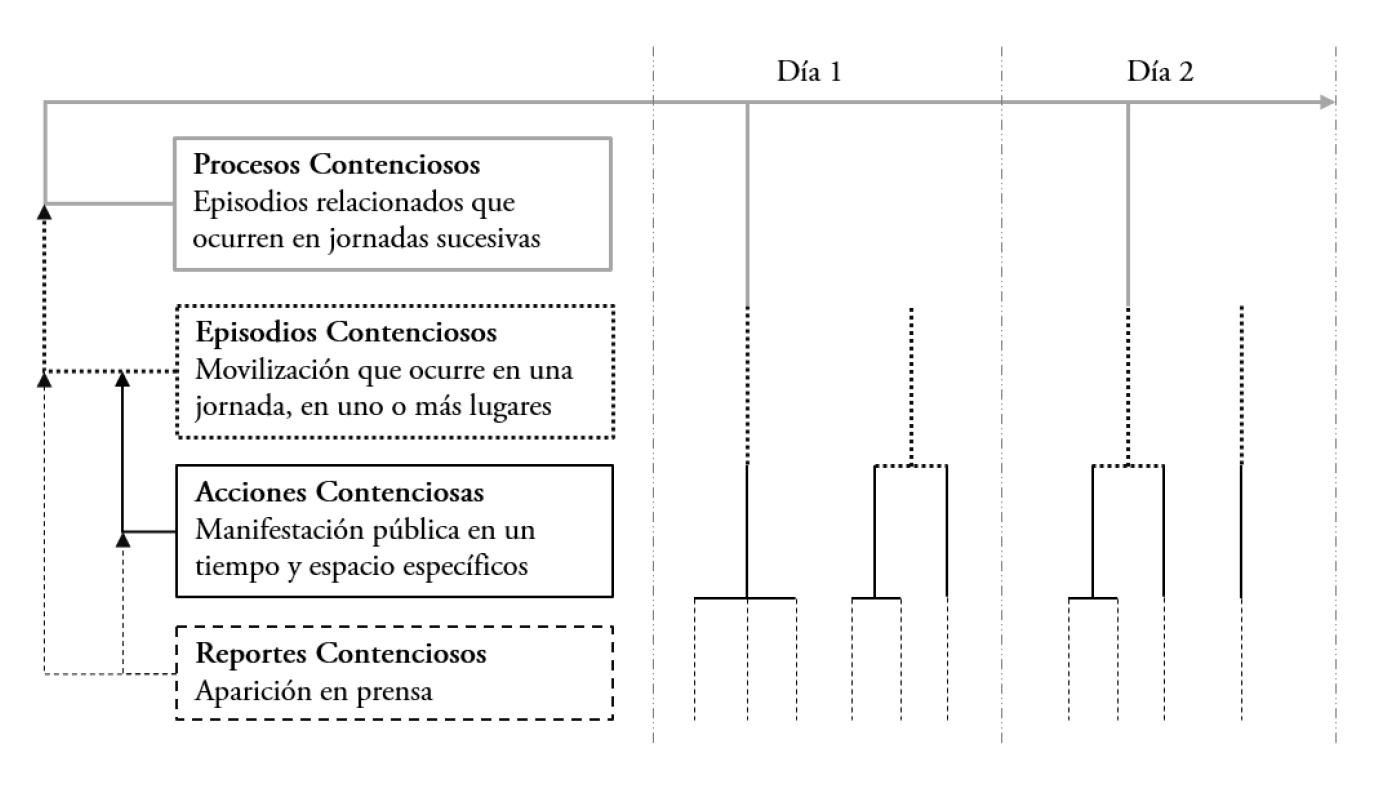
\includegraphics[width=0.8\linewidth,]{user} 

}

\caption{Niveles de observación del conflicto social}\label{fig:fig1}
\end{figure}

Las principales actividades del Observatorio de Conflictos se centran en
la mantención, mejora y ampliación de esta base de datos, así como
también en la generación de análisis a partir de la misma. Por tanto, el
desarrollo de la práctica profesional se enfocó en tales objetivos,
desempeñando tareas de recolección de información, codificación de
información, manipulación y análisis de datos, y elaboración de
documentos de trabajo para el Observatorio que se detallan en la
siguiente sección.

\hypertarget{actividades-observatorio-de-conflictos}{%
\subsection{2. Actividades Observatorio de
Conflictos}\label{actividades-observatorio-de-conflictos}}

\hypertarget{a-recolecciuxf3n-y-sistematizaciuxf3n-de-informaciuxf3n}{%
\subsubsection{a) Recolección y sistematización de
información}\label{a-recolecciuxf3n-y-sistematizaciuxf3n-de-informaciuxf3n}}

\doublespacing

Una de las principales actividades del Observatorio de Conflictos
corresponde a la recolección y sistematización de información mediante
la revisión de prensa. Esta es una tarea diaria que se rige bajo un plan
metodológico riguroso (AEP) para identificar eventos contenciosos que
luego son ordenados y posteriormente codificados. Estos lineamientos se
basan en tres criterios análiticos consecutivos: i) identificar una
noticia en un medio de prensa online o escrito a partir de la definición
de acción contenciosa establecida por el Observatorio, ii) definir que
la noticia contenga la información mínima para ser recolectada, esto es,
la descripción de un evento de protesta que implique un conflicto -una
relación de oposición entre al menos dos partes-, un lugar y una fecha,
y iii) determinar el nivel de observación del conflicto a partir de la
Figura 1. Si la noticia reúne las condiciones descritas pasa a ser
recolectada y sistematizada en orden cronológico en documentos
compartidos por los miembros del Observatorio. Además, cada evento que
es recolectado es también fotografiado y guardado en el registro del
Observatorio, siendo utilizado posteriormente para la consolidación de
la base de datos mediante la revisión cruzada entre codificadores sobre
un remuestreo del 10\% de los casos totales de la base.

\begin{figure}[!ht]

{\centering 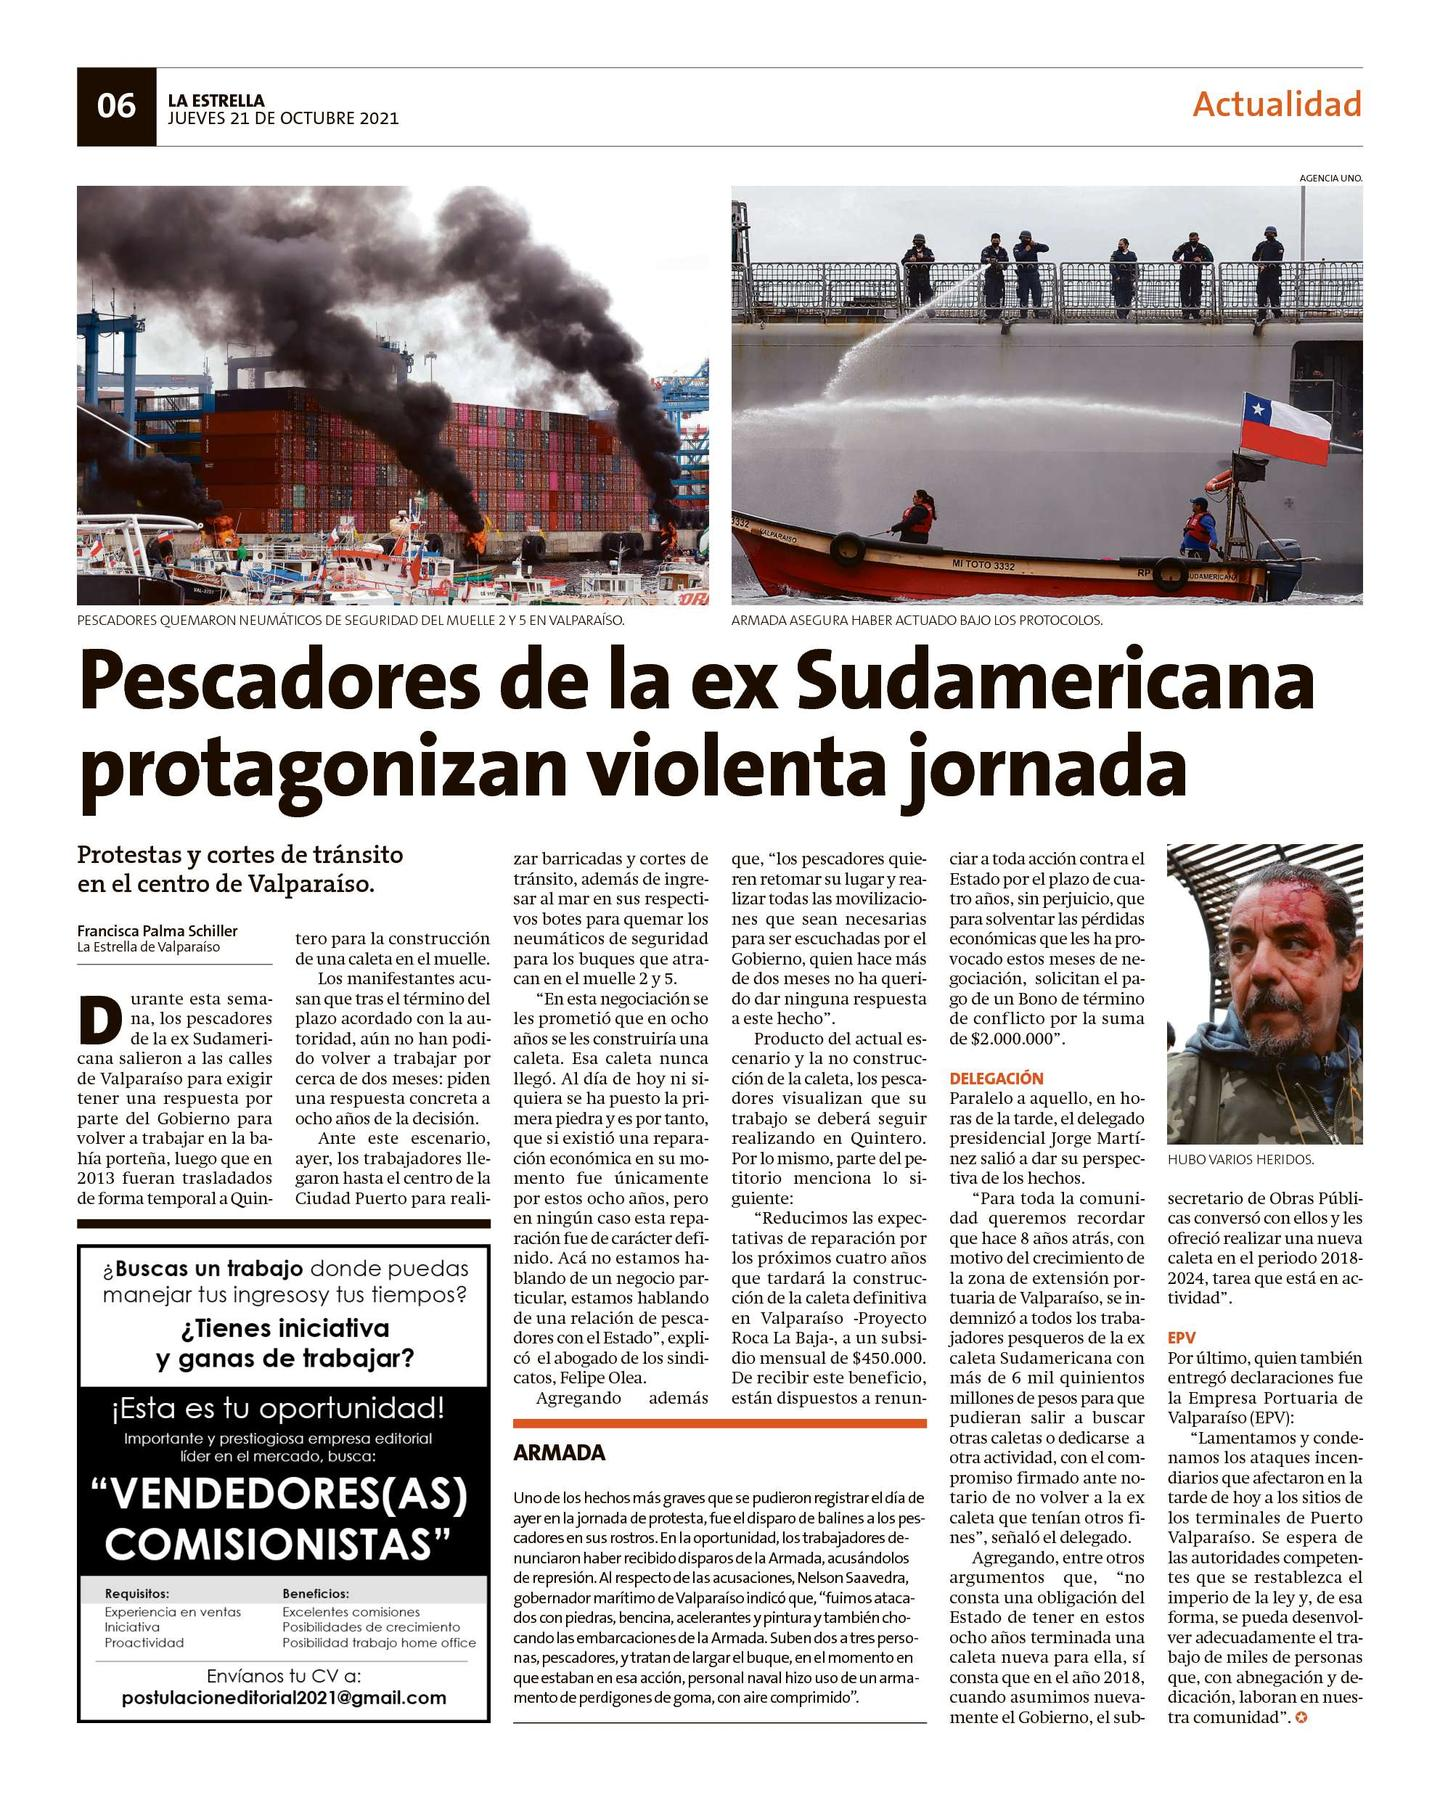
\includegraphics[width=0.6\linewidth,]{val} 

}

\caption{Ejemplo recolección online medio La Estrella de Valparaíso}\label{fig:fig2}
\end{figure}

La recolección de información se realiza de dos maneras. Por un lado, se
revisan los medios de prensa seleccionados en formato online para el año
2021. Como practicante, me correspondió revisar un total de 5 medios de
prensa online: La Estrella de Arica, La Estrella de Valparaíso,
Cooperativa, El Divisadero y El Rancagüino. Esta revisión se realiza
mediante una búsqueda web de los respectivos medios abarcando rangos de
información mensual. En el caso de los dos primeros diarios, la revisión
documental es manual debido a la disponibilidad virtual del diario (ver
Figura 2 de ejemplo). Mientras que para los demás diarios, se utilizan
las herramientas de Google Site para la revisión. Además de la revisión
de medios para el 2021 y gracias a un convenio establecido entre el
Diario Cooperativa y el Observatorio de Conflictos, se facilitó el
portal web de este medio de prensa para recolectar noticias de eventos
contenciosos entre los años 2010 y 2009. Esto se debe a que actualmente
la base de datos del Observatorio no contiene información de acciones
contenciosas para dichos años en tal medio, siendo uno de los
inconvenientes de la base de datos a la hora de realizar análisis
comparables con la serie completa. Así, con el objetivo de ampliar la
base de datos, se recolectan noticias de eventos de protesta en el
portal web del diario Cooperativa entre el 2010 y 2009, pasando por el
mismo proceso metodológico descrito anteriormente.

Por otro lado, se revisan los medios de prensa seleccionados en formato
impreso para el año 2007 en la Biblioteca Nacional de Chile. Como
practicante, me correspondió revisar un total de 7 medios de prensa
impresos: La Estrella de Arica, La Estrella de Antofagasta, La Región de
Coquimbo, El Rancagüino, Austral de Temuco, Austral de Valdivia y Diario
Financiero. Todos estos diarios son revisados manualmente en la
Biblioteca Nacional. Para algunos casos solo fue necesario hacer el
registro (fotografiar), mientras que para la mayoría de los diarios se
realiza tanto la recopilación como el registro de acuerdo a las
instrucciones metodológicas del Observatorio (ver Figura 3 de ejemplo).
Nuevamente, con el propósito de expandir la base de datos en términos
temporales, se recopila información de acciones contenciosas para los
años 2007 y 2006. Además, el objetivo a largo plazo de esta actividad es
que, una vez finalizada, se puedan realizar análisis que contrasten la
dinámica de las acciones contenciosas en Chile antes y después del
``resurgimiento'' de la política contenciosa y los ciclos de protestas
que datan desde el 2008 hacia adelante
(\protect\hyperlink{ref-sommaSocialMovementsLatin2020}{Somma, 2020}).

\begin{figure}[!ht]

{\centering 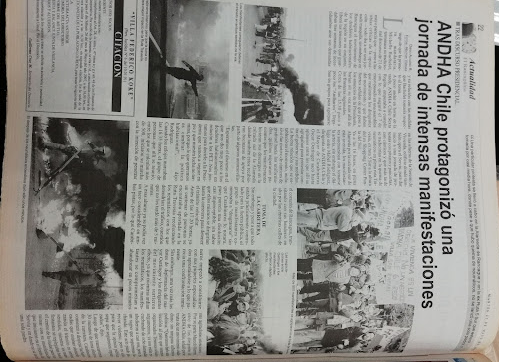
\includegraphics[width=0.8\linewidth,]{biblio} 

}

\caption{Ejemplo recolección impresa medio El Rancagüino}\label{fig:fig3}
\end{figure}

\hypertarget{b-codificaciuxf3n-de-informaciuxf3n}{%
\subsubsection{b) Codificación de
información}\label{b-codificaciuxf3n-de-informaciuxf3n}}

\doublespacing

La segunda de las actividades principales del Observatorio corresponde a
la codificación de la información recolectada mediante el análisis de
prensa. Esta es una actividad diaria que se realiza en paralelo a la
recolección de noticias, logrando un ritmo de trabajo en donde se
recolecta y codifica en una misma oportunidad. Metodológicamente, la
codificación se rige bajo un Code Sheet que contiene un conjunto de
indicaciones necesarias para codificar los datos que se requieren. A
esto se le suma la realización de una capacitación a los practicantes
sobre el proceso de codificación por parte de los miembros del
Observatorio. Como practicante, me correspondió codificar únicamente la
información recolectada de los medios online nombrados anteriormente.
Las dimensiones de análisis que son codificadas se alinean con los
objetivos propuestos por el Observatorio, abarcando elementos como: la
cantidad de acciones contenciosas, el lugar y momento en el que
ocurrieron, la cantidad de participantes, los actores involucrados
entendidos como demandantes y demandados, la(s) institución(es) o
entidad(es) a las que se dirige la protesta, los actores sociales
presentes (trabajadores, estudiantes, pueblos indígenas entre otros),
las organizaciones convocantes que son nombradas, las demandas presentes
en la protesta (laborales, estudiantiles, ambientalistas entre otras),
los campos de conflictividad a los que corresponden los eventos, las
tácticas de protesta empleadas (pacíficas, disruptivas o violentas), la
presencia policial y la existencia de enfrentamientos, arrestos, heridos
y muertos. Esta codificación se elabora en un archivo Excel compartido
entre los miembros del Observatorio. Cada medio tiene su respectiva
codificación, y una vez terminados se realizan revisiones cruzadas entre
los codificadores de un remuestreo del 10\% de los casos totales con el
fin de verificar que los criterios utilizados en la codificación sean
los mismos y así consolidar la base de datos.

\hypertarget{c-manipulaciuxf3n-y-anuxe1lisis-de-datos}{%
\subsubsection{c) Manipulación y análisis de
datos}\label{c-manipulaciuxf3n-y-anuxe1lisis-de-datos}}

\doublespacing

Una tercera actividad desarrollada en el Observatorio de Conflictos es
la manipulación y análisis de los datos contenidos en la base. Esto, con
el objetivo de ser utilizados en los informes anuales del Observatorio y
puesta en formato público para el libre acceso. Concretamente, como
practicante tuve que realizar tareas de recodificación de datos,
creación de variables de texto, etiquetado de variables y valores además
de revisar y comparar la distribución univariada y bivariada de los
datos para la serie 2009-2020. Lo anterior fue realizado mediante el
software R, siendo uno de los requerimientos de la institución puesto
que, hasta el momento, solo se utilizaba el software SPSS, quedando así
como un primer insumo reproducible para la futura ampliación de la base
de datos. El producto de esta actividad es la primera base de datos del
Observatorio de Conflictos procesada y etiquetada en formato RData., la
cual posteriormente formará parte del Dataverse de COES en la web de la
Harvard University.

\hypertarget{d-elaboraciuxf3n-de-documentos-reproducibles-y-abiertos}{%
\subsubsection{d) Elaboración de documentos reproducibles y
abiertos}\label{d-elaboraciuxf3n-de-documentos-reproducibles-y-abiertos}}

\doublespacing

Por último, y con el propósito de fomentar la política de apertura de
datos e investigación propuesta por COES como por el propio
Observatorio, se elaboraron dos documentos de manipulación y uso de la
base de datos en formato público y reproducible. Para generar ambos
documentos se utilizó la plataforma Github para trabajo colaborativo y
abierto, creando un usuario del Observatorio que almacena los
repositorios en donde se alojan estos documentos hechos en software R.
El primer documento corresponde a un manual que enseña cómo manipular y
visualizar los datos del Observatorio en Rstudio (ver Figuras 4 y 5 de
ejemplos). Si bien este manual tiene por primer objetivo el ilustrar al
público general sobre cómo usar y graficar variables de la base de datos
del Observatorio, también pretende ser un primer insumo que familiarice
a los mismos integrantes del Observatorio sobre la manipulación de datos
en R. Así también, un segundo objetivo de este documento es que sirva
como base para que el Observatorio pueda crear sitios web con
aplicaciones interactivas (Shiny Apps) que permitan manipular y exportar
datos de manera sencilla y pública. Este manual se encuentra finalizado
y publicado en la plataforma RPubs para su acceso\footnote{\url{https://rpubs.com/Andreas-Lafferte/visualization-coes}}.

\begin{figure}[!ht]

{\centering 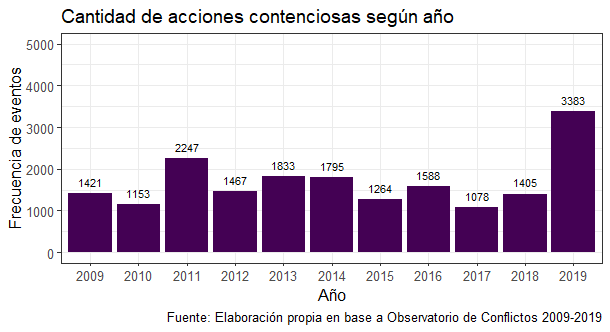
\includegraphics[width=0.9\linewidth,]{plot1} 

}

\caption{Ejemplo de gráfico evolución cantidad de acciones contenciosas 2009-2019}\label{fig:fig4}
\end{figure}

El segundo documento corresponde a un libro de códigos de la base de
datos del Observatorio de Conflictos. Apuntando a la masificación del
uso de los datos del Observatorio, se me encomienda la tarea de generar
un libro de códigos de la base de datos mediante el software R y el
paquete `codebook.' Este libro de códigos busca suplir la ausencia de un
documento metodológico que describa las variables contenidas en la base
de datos del Observatorio, además de ser un documento público,
interactivo y de fácil manejo para investigadores e investigadoras. Este
libro de códigos se encuentra finalizado y publicado en la plataforma
RPubs para su libre acceso\footnote{\url{https://rpubs.com/Andreas-Lafferte/codebook-oc}},
y posteriormente será enlazado al Dataverse de COES en la web de la
Harvard University.

\begin{figure}[!ht]

{\centering 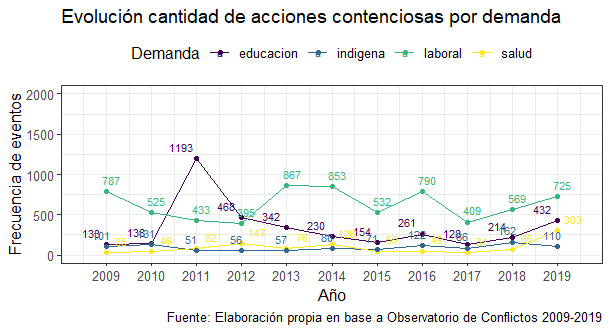
\includegraphics[width=0.9\linewidth,]{plot2} 

}

\caption{Ejemplo de gráfico evolución cantidad de acciones contenciosas según demanda 2009-2019}\label{fig:fig5}
\end{figure}

\hypertarget{principales-problemas-identificados}{%
\subsection{3. Principales problemas
identificados}\label{principales-problemas-identificados}}

\doublespacing

Los principales obstáculos encontrados en la institución para
desarrollar las actividades anteriormente descritas son mínimos, aunque
pueden destacarse particularmente dos. En primer lugar, y si bien no es
algo que dependa de la institución, la tarea de recolección de noticias
impresas en la Biblioteca Nacional se ha visto truncada por la situación
sociosanitaria del país. Esto ha implicado que dicha tarea de
recolección se haya retrasado gran parte de este semestre, logrando
comenzar a realizarce recien a fines del mes de octubre. Además, debido
a las propias lógicas de funcionamiento y cuidado de la Biblioteca
Nacional, tanto la asistencia a la Biblioteca como la solicitud del
material de prensa es restringido, implicando que esta labor no se
desarrolle regularmente. En segundo lugar, se encontraron algunas
dificultades relacionadas con aspectos específicos de la organización
del trabajo dentro de la institución. Por un lado, debido a la
naturaleza de la práctica profesional y a los objetivos del
Observatorio, se facilitaba la realización de múltiples tareas al mismo
tiempo. En específico, al no existir un ordenamiento de actividades
prioritarias dentro del Observatorio y debido a que el trabajo se
organiza por la obtención de productos, la jornada de trabajo se
distribuía en múltiples tareas simultáneas
(recolección/codificación/manipulación de datos entre otras) que
terminaban desorientando a los practicantes sobre qué era lo prioritario
o esencial en términos de plazos. Por otro lado, y en relación a esto
último, la otra dificultad encontrada en la institución fue la ausencia
de planes o plazos definidos para la organización del trabajo y la
entrega de los productos solicitados, lo cual devino en confusiones para
los practicantes y, en determinados ocasiones afectó el rendimiento y
calidad del trabajo. Sin embargo, estas dificultades fueron conversadas
al interior del Observatorio a solicitud de los practicantes, llegando a
buen puerto con una solución de jerarquización de tareas y planteamiento
de plazos.

\hypertarget{evaluaciuxf3n-de-la-formaciuxf3n-entregada-por-la-carrera-de-sociologuxeda}{%
\subsection{4. Evaluación de la formación entregada por la carrera de
Sociología}\label{evaluaciuxf3n-de-la-formaciuxf3n-entregada-por-la-carrera-de-sociologuxeda}}

\doublespacing

La formación entregada por la carrera de Sociología resultó ser
sumamente útil para el desarrollo de la práctica profesional, resaltando
en dos aspectos: uno teórico y otro metodológico. No obstante lo
anterior, a partir de la experiencia profesional en esta institución se
pueden destacar ciertos aspectos a profundizar en la formación académica
de la carrera que pueden ser de utilidad para futuros egresados. A
continuación, se exponen los principales aportes teóricos y
metodológicos brindados por la carrera de Sociología para el desempeño
de esta práctica profesional, así como también ciertas recomendaciones a
considerar.

En primer lugar, las diversas herramientas y conocimientos teóricos
adquiridos durante la carrera fueron fundamentales para la comprensión
del objeto de estudio del Observatorio, esto es, el conflicto social.
Por un lado, pueden destacarse los aportes de la teoría sociológica por
sí misma. Las perspectivas clásicas para comprender los motivos y
definir al conflicto social de autores como Marx
(\protect\hyperlink{ref-marxCapital1975}{1975}) y Simmel
(\protect\hyperlink{ref-simmelGeorgSimmelIndividuality2011}{2011})
resultaron relevantes para observar la conflictividad social chilena en
la actualidad, especialmente en lo a que los motivos y dinámicas del
conflicto refieren
(\protect\hyperlink{ref-oberschallTheoriesSocialConflict1978}{Oberschall,
1978}). Así también, más importante aún fueron los aportes más modernos
de la teoría del conflicto que derivan de los postulados clásicos, como
lo son el marco interpretativo del conflicto de Collins
(\protect\hyperlink{ref-collinsConflictSociologySociological2009a}{2009})
o Dahrendorf
(\protect\hyperlink{ref-dahrendorfTheorySocialConflict1958a}{1958})
desde una sociología más weberiana, los postulados del funcionalismo con
Lewis Coser
(\protect\hyperlink{ref-coserSocialConflictTheory1957a}{1957}), o las
miradas materialistas del conflicto con Tilly y Tarrow
(\protect\hyperlink{ref-tillyContentiousPolitics2015a}{2015}). Por otro
lado, cabe mencionar los aportes de la sociología política y la
literatura de los movimientos sociales. Desde los giros
``post-materialistas'' con autores como Touraine
(\protect\hyperlink{ref-touraineIntroductionStudySocial1985}{1985}) o
Melucci
(\protect\hyperlink{ref-melucciSymbolicChallengeContemporary1985}{1985}),
hasta el resurgimiento de la política contenciosa y los conflictos
redistributivos en Europa
(\protect\hyperlink{ref-dellaportaSocialMovementsIntroduction2006}{Della
Porta \& Diani, 2006}) y América Latina
(\protect\hyperlink{ref-donosoSocialMovementsChile2017a}{Donoso \& von
Bülow, 2017};
\protect\hyperlink{ref-sommaSocialMovementsLatin2020}{Somma, 2020}),
estos cursos sirvieron para poder identificar y comprender las
características que han adquirido los movimientos y conflictos sociales
en las últimas décadas. De tal modo, tanto los aportes de la teoría
sociológica como los aportes de los cursos sobre historia social,
sociología política y movimientos sociales fueron centrales para
comprender las distintas perspectivas y consensos sobre el conflicto
social, permitiendo que el desarrollo de la práctica profesional fuera
más óptimo al poseer distintas herramientas teóricas para examinar el
objeto de estudio.

En segundo lugar, las herramientas y conocimientos metodológicos
entregados por la carrera resultaron centrales para el desempeño de las
actividades en la práctica profesional. Desde una vereda cuantitativa,
los cursos al respecto aportan con los saberes y habilidades necesarias
para el campo laboral. En específico, durante esta práctica profesional
tuve la oportunidad de construir una base de datos a partir de una
metodología de análisis de eventos de protesta (AEP) en diversos medios
de prensa. A este respecto, no haber contado con cursos como
Metodologías Cuantitativas hubiera dificultado enormemente la generación
de indicadores, la comprensión del ejercicio de medición, la
clasificación de variables y la formulación de diseños de investigación.
Asimismo, los cursos de estadística impartidos por la carrera fueron más
que claves en, al menos, dos direcciones: por un lado, para contar con
los conocimientos estadísticos necesarios para realizar los análisis
requeridos por la institución y, por el otro, para contar con una
intensa experiencia en la manipulación y análisis de datos en el
software Rstudio. Por último y no menos importante, fueron sumamente
útiles los conocimientos entregados por el curso de Ciencia Social
Abierta de la carrera. Este tipo de herramientas son de algún modo
escasas, por lo que contar con ellas permitieron abrir nuevas opciones y
actividades dentro del Observatorio, tales como la apertura de datos e
investigación, la generación de documentos libres y reproducibles, el
trabajo colaborativo e incluso el desarrollo de sitios web. Con todo,
los saberes y herramientas metodológicas transmitidas por la carrera
fueron determinantes para el desarrollo de esta práctica profesional.

Ahora bien, a pesar de que la formación de la carrera en términos
teóricos y metodológicos fueron fundamentales, también hay algunos
aspectos que pueden ser potenciados para el beneficio de los futuros
egresados en Sociología. En el desarrollo de esta práctica profesional
tuve que aplicar conocimientos que fueron aprendidos por fuera de la
carrera, aunque tomando como base lo aportado por la misma. En
específico, cursos de ciencia abierta y manipulación de datos deberían
potenciarse. Como se mencionó, las habilidades entregadas por el curso
de Ciencia Social Abierta no solo fueron útiles para las tareas del
Observatorio, sino que aportaron una ventaja comparativa relevante
dentro del mismo y, posiblemente, dentro del ámbito laboral en la
disciplina. De tal modo, potenciar más cátedras en esta materia con
nuevos tópicos y modalidades aportarían al perfil metodológico de los
futuros egresados. Así también, puede resultar provechoso que la carrera
imparta cursos dedicados exclusivamente a la manipulación de datos ya
que no es el objetivo central de los cursos de estadística. En este
sentido, potenciar cursos como el de Ciencias Sociales Computacionales o
vincular cátedras similares de otras facultades a la carrera son
fundamentales para los requerimientos del mercado laboral en la
actualidad y el desarrollo de la investigación empírica.

\hypertarget{evaluaciuxf3n-de-los-aprendizajes-adquiridos}{%
\subsection{5. Evaluación de los aprendizajes
adquiridos}\label{evaluaciuxf3n-de-los-aprendizajes-adquiridos}}

\doublespacing

Los aprendizajes adquiridos durante el desarrollo de esta práctica
profesional son de orden principalmente metodológico. Por un lado, se
puede mencionar la aplicación de técnicas de recolección y revisión
documental en el Observatorio, siendo una experiencia totalmente nueva y
un gran aporte para el futuro profesional. Por otro lado, destaca el uso
de metodologías rigurosas e innovadoras para la construcción de datos.
En detalle, el análisis de eventos de protestas (AEP) mediante el
análisis de prensa me permitió expandir mis conocimientos sobre la
generación o recolección de datos, así como también en la construcción
de indicadores. Además, aporta con una buena primera experiencia en la
introducción de metodologías que son comúnmente utilizadas en ámbitos de
investigación sobre los movimientos sociales, la participación en
protestas y la desigualdad política. Por último, la pasada en esta
institución también me brindó la posibilidad de profundizar mis
conocimientos y habilidades en la manipulación, análisis y visualización
de datos utilizando software estadísticos de código abierto, todo ello
con el fin de generar insumos tanto para el propio Observatorio de
Conflictos como para el público general mediante documentos abiertos y
reproducibles.

\hypertarget{referencias-bibliogruxe1ficas}{%
\subsection{Referencias
bibliográficas}\label{referencias-bibliogruxe1ficas}}

\doublespacing

\hypertarget{refs}{}
\begin{CSLReferences}{1}{0}
\leavevmode\hypertarget{ref-coesManualMetodologicoObservatorio2018}{}%
COES. (2018). \emph{{Manual Metodológico Observatorio de Conflictos}}.
98.

\leavevmode\hypertarget{ref-collinsConflictSociologySociological2009a}{}%
Collins, R. (2009). \emph{Conflict {Sociology}: {A Sociological Classic
Updated}} (Abridged and updated). {Paradigm Publishers}.

\leavevmode\hypertarget{ref-coserSocialConflictTheory1957a}{}%
Coser, L. A. (1957). Social {Conflict} and the {Theory} of {Social
Change}. \emph{The British Journal of Sociology}, \emph{8}(3), 197.
\url{https://doi.org/10.2307/586859}

\leavevmode\hypertarget{ref-dahrendorfTheorySocialConflict1958a}{}%
Dahrendorf, R. (1958). Toward a {Theory} of {Social Conflict}.
\emph{Journal of Conflict Resolution}, \emph{2}(2), 170--183.
\url{https://doi.org/10.1177/002200275800200204}

\leavevmode\hypertarget{ref-dellaportaSocialMovementsIntroduction2006}{}%
Della Porta, D., \& Diani, M. (2006). \emph{Social movements: An
introduction} (2nd ed). {Blackwell Publishing}.

\leavevmode\hypertarget{ref-donosoSocialMovementsChile2017a}{}%
Donoso, S., \& von Bülow, M. (Eds.). (2017). \emph{Social {Movements} in
{Chile}}. {Palgrave Macmillan US}.
\url{https://doi.org/10.1057/978-1-137-60013-4}

\leavevmode\hypertarget{ref-joignantInformeAnualObservatorio2020}{}%
Joignant, A., Garretón, M., Somma, N. M., \& Campos, T. (2020).
\emph{{Informe Anual Observatorio de Conflictos 2020}}. 98.

\leavevmode\hypertarget{ref-kriesbergConstructiveConflictsEscalation2012}{}%
Kriesberg, L., \& Dayton, B. W. (2012). \emph{Constructive conflicts:
From escalation to resolution} (4th ed). {Rowman \& Littlefield}.

\leavevmode\hypertarget{ref-marxCapital1975}{}%
Marx, K. (1975). \emph{El capital: Crítica de la economía política.
{Tomo I} / {Vol}. {I El} proceso de producción del capital}. {Siglo
XXI}.

\leavevmode\hypertarget{ref-melucciSymbolicChallengeContemporary1985}{}%
Melucci, A. (1985). The {Symbolic Challenge} of {Contemporary
Movements}. \emph{Social Research}, \emph{52}(4), 789--816.

\leavevmode\hypertarget{ref-oberschallTheoriesSocialConflict1978}{}%
Oberschall, A. (1978). \emph{Theories of {Social Conflict}}. 25.

\leavevmode\hypertarget{ref-simmelGeorgSimmelIndividuality2011}{}%
Simmel, G. (2011). \emph{Georg {Simmel} on {Individuality} and {Social
Forms}}. {University of Chicago Press}.

\leavevmode\hypertarget{ref-sommaSocialMovementsLatin2020}{}%
Somma, N. M. (2020). Social {Movements} in {Latin AmericaMapping} the
{Literature}. In \emph{The {Oxford Handbook} of the {Sociology} of
{Latin America}} (pp. 303--324). {Oxford University Press}.
\url{https://doi.org/10.1093/oxfordhb/9780190926557.013.20}

\leavevmode\hypertarget{ref-tillyContentiousPolitics2015a}{}%
Tilly, C., \& Tarrow, S. G. (2015). \emph{Contentious {Politics}}
(Second revised edition). {Oxford University Press}.

\leavevmode\hypertarget{ref-touraineIntroductionStudySocial1985}{}%
Touraine, A. (1985). An {Introduction} to the {Study} of {Social
Movements}. \emph{Social Research}, \emph{52}(4,), 749--787.

\end{CSLReferences}

\end{document}
